\documentclass[12pt]{article}
\usepackage{geometry}                % See geometry.pdf to learn the layout options. There are lots.
\geometry{a4paper}                   % ... or a4paper or a5paper or ...
%\geometry{landscape}                % Activate for for rotated page geometry
\usepackage[parfill]{parskip}    % Activate to begin paragraphs with an empty line rather than an indent
\usepackage{enumitem}
\usepackage{graphicx}
\usepackage{amssymb}
\usepackage{amsmath}
\usepackage{cancel}
\usepackage{epstopdf}
\DeclareGraphicsRule{.tif}{png}{.png}{`convert #1 `dirname #1`/`basename #1 .tif`.png}
\usepackage{breqn}
\usepackage{float}
\usepackage{breqn}

\title{Econ 210C Problem Set \# 4}
\author{Churn Ken Lee}
%\date{}                                           % Activate to display a given date or no date

\begin{document}




\maketitle

\section{Labor supply problem}
An individual with time-separable utility has first order conditions
\begin{align*}
\frac{1}{C_t} &= \lambda_t  \\
\lambda_t w_t &= \frac{1}{1-L_t} 
\end{align*}
while an individual with non-separable preferences has first order conditions
\begin{gather*}
\frac{1}{C_t} = \lambda_t  \\
\lambda_t w_t = \frac{0.5}{1 - 0.5 \left( L_t + L_{t-1} \right)} + \beta \frac{0.5}{1 - 0.5 \left( L_{t+1} + L_t \right)}
\end{gather*}
\subsection*{(a)}
	Since investment is impossible, $w_t L_t = C_t$ always, so separable utility implies 
	\begin{equation*}
	L_t = \frac{1}{2}
	\end{equation*}
	which does not allow for any response to shocks. 
	With non-separable preferences, we have:
	\begin{equation*}
	\frac{w_t}{C_t}  = \frac{0.5}{1 - 0.5 \left( L_t + L_{t-1} \right)} + \beta \frac{0.5}{1 - 0.5 \left( L_{t+1} + L_t \right)}
	\end{equation*}
	so individuals adjust their labor supply in neighboring periods when a shock is expected (so they work less when the return is lower).
	Labor supply changes are larger in the non separable case. 
	
\subsection*{(b)} 
Labor supply is perfectly inelastic for separable preferences; the labor supply elasticity is higher in the non separable case. 

\section{Demand shock}

\subsection*{(a)}

The consumption-leisure condition at time $t$ is just equating marginal benefits of labor and leisure $\frac{W_t}{C_t} = v_t L_t^\chi$.

\subsection*{(b)}

The consumer consuming one less unit today means they are losing out on $\frac{1}{C_t}$ today. 
With that, they can buy $\frac{1}{P_t}$ units of capital today, and tomorrow they will get $P_{t+1} + d_{t+1}$ from that unit of capital. 
So their payoff tomorrow is 
\[
\frac{1}{P_t} \times (P_{t+1} + d_{t+1}) \times \frac{\beta}{C_{t+1}}
\]
and optimality therefore implies we have
\[
\frac{1}{C_t} = \frac{1}{P_t} \times (P_{t+1} + d_{t+1}) \times \frac{\beta}{C_{t+1}}
\]
as the inter-temporal optimality condition.

\subsection*{(c)}

The price of capital is such that $K_t^s = \bar{K}$, constrained by the Euler equation.

\subsection*{(e)} 
We have
	\begin{equation*}
	L_t = \left( \frac{\lambda_t W_t}{\nu_t} \right)^{\frac{1}{\chi}}
	\end{equation*}
	so $\nu_t$ is a labor disutility shock, with higher values of $\nu_t$ meaning more disutility of labor supply, and therefore lower labor suppky. 
	When $\chi = 1$, we have the labor supply curve 
	\begin{equation*}
	W_t = \frac{\nu_t}{\lambda_t} L_t = \nu_t C_t L_t  
	\end{equation*}
	showing that a positive $\nu_t$ shock steepens the labor supply curve. 
	
	\subsection*{(e)} Strongly countercyclical $\nu_t$ allows countercyclical real wages when consumption and labor supply are procyclical, so the issue that the RBC model has of highly procyclical wages can be addressed, though it seems almost like an epicycle.


\section{Business cycle and external returns to scale}

\subsection*{(a)}

Each firm sets wage equal to marginal product of labor, so we have
\[
W_t = Y_t^{1-1/\gamma} \left(\frac{K_{it}}{L_{it}}\right)^{\alpha} Z_t^{1-\alpha}
\]
and substituting back in we have
\[
W _ { t } = ( 1- \alpha ) \frac{Y_{i,t}}{L_{i,t}}
\]
\subsection*{(b)}

\begin{align*}
	Y_t &= \int_{0}^{1} E_t K_{i,t}^\alpha \left( Z_t L_{i,t} \right)^{1-\alpha} di \\
	& = E_t Z_t^{1-\alpha} \int_{0}^{1} K_{i,t}^\alpha  L_{i,t}^{1-\alpha} di \\
	& = E_t K_t^\alpha (Z_t L_t)^{1-\alpha}
	\end{align*}
	Substitute $E_t = Y_t^{1- \frac{1}{\gamma}}$, and we have increasing returns to scale at the aggregate level
	\begin{equation*}
	Y _ { t } = \left[ K _ { t } ^ { \alpha } \left( Z _ { t } L _ { t } \right) ^ { 1- \alpha } \right] ^ { \gamma }
	\end{equation*}
	with social labor demand curve
	\[
	W _ { t } = \gamma ( 1- \alpha ) Y _ { t } L _ { t } ^ { - 1}
	\] and no economic profit without imperfect competition. 

\subsection*{(c)}
A negative $\nu_t$ shock implies labor supply increases. 
The implied increased income means consumption increases. 
Social labor demand is flatter, and we can calibrate the externality to match empirical wage increases (with the externality moderate enough to get a downward slope).
Average labor productivity is procyclical because it increases with real wages. 

\subsection*{(d)}
 $\gamma = 1$ gives a standard RBC model that does not have a flattened social labor demand curve, which has the puzzle that real wages and labor productivity are too procyclical. 
 
 \subsection*{(e)}
 The statement is correct; in a standard RBC model strong procyclicality of wages is inevitable. 
 The researcher might use $\nu_t$ shocks that are negatively correlated with technology shocks to get a flatter labor supply curve and smaller volatility for wages with larger volatility for aggregate labor. 
A change in preferences across all agents in the real world seems quite implausible.	If $\gamma > 1$, we can calibrate the externality to get the mildly procyclical wage and labor productivity needed. 


\section{Problems from Romer}
\subsection{Problem 6.10}

\subsubsection*{(a)} We just solve the system for $p, p^{*}$, and $y$ to get 
	\begin{align*}
	p & = \frac{f \phi m'}{1 - f + f\phi} \\
	p^{*} & = \frac{\phi m'}{1 - f + f\phi} \\
	y & = \frac{m' (1-f)}{1 - f + f\phi}
	\end{align*}
	
	\subsubsection*{(b)} The plots are shown in Figure \ref{misclabel}.
	\begin{figure}[htbp]
        \begin{center}
        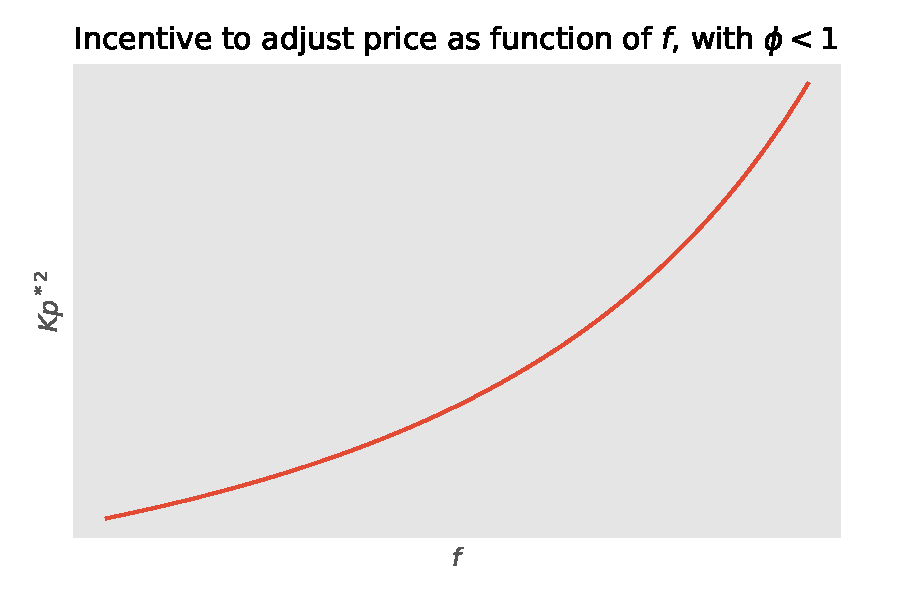
\includegraphics[scale = 0.4]{phi_less_than_one}
        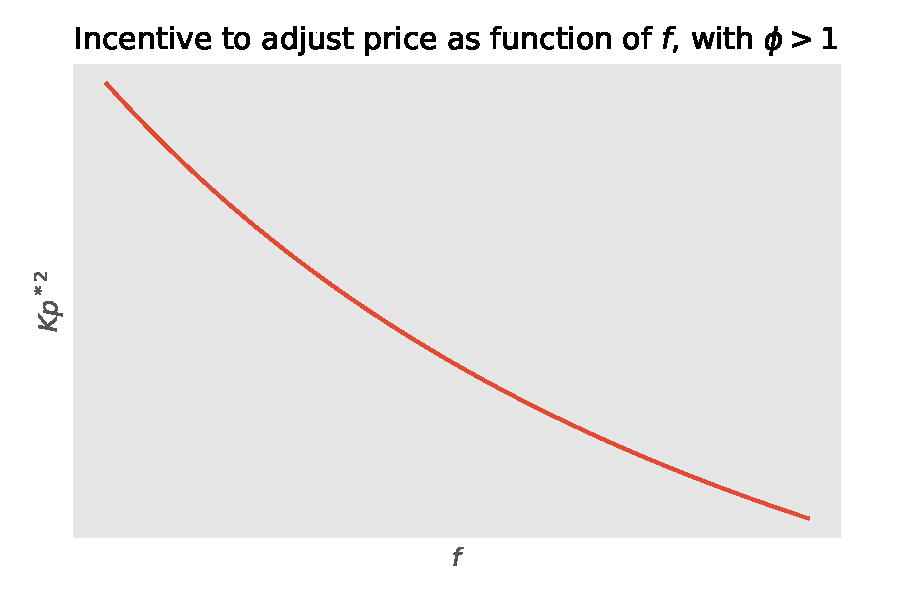
\includegraphics[scale = 0.4]{phi_greater_than_one}
        \caption{6.10(b)}
        \label{misclabel}
        \end{center}
    \end{figure}

	
	
	\subsubsection*{(c)} Whether a firm adjusts its price is a function of$Z$. 
	Assume that $\phi <1$ and suppose the menu cost is lower than the incentive of a firm when no other firm is adjusting their prices, then all firms adjusting their prices is the only Nash equilibrium. 
	
	When the menu cost is higher than the incentive of a firm when all the other firms are adjusting their prices, no price adjustment is the only Nash equilibrium. 
	
	In the intermediate case $Z = K p^{*} (f)$ for some $f$, and a fraction $f$ of the firms adjusting their prices is the only Nash equilibrium, because for $f' \neq f$ some firms have an incentive to deviate. 

\subsection{Problem 6.11}

\subsubsection*{(a)}
If the firm does not adjust its price it has profit $\pi \left( y_1, r^{*}(y_0)  \right)$ as compared to $\pi \left( y_1, r^{*}(y_1)  \right)$ when adjusting. 
The difference between these two is the potential gain from and therefore the incentive to engage in a price adjustment.
Smaller $G$ implies stickier prices (because adjustments are more rare). 

\subsubsection*{(b)}

We have
\[
\frac{\partial G}{\partial y_1} = \pi_1(y_1, r^*(y_1)) + \pi_2(y_1, r^*(y_1)) \cdot \frac{\partial r^*(y_1)}{\partial y_1} - \pi_1(y_1, r^*(y_0))
\]
but since $\pi_2(y_0, r^*(y_0)) = 0$ characterizes $r^*$, we have that this is zero when evaluated at $y_0$.

Now we have
\begin{tiny}
\begin{align*}
\frac{\partial^2 G}{\partial y_1^2} = \pi_{11}(y_1, r^*(y_1))  &+ \pi_{12}(y_1, r^*(y_1)) \frac{\partial r^*(y_1)}{\partial y_1} + \left(\pi_{21}(y_1, r^*(y_1)) + \pi_{22}(y_1, r^*(y_1)) \frac{\partial r^*(y_1)}{\partial y_1} \right) \frac{\partial r^*(y_1)}{\partial y_1} \\&+ \pi_2(y_1, r^*(y_1)) \cdot \frac{\partial^2 r^*(y_1)}{\partial y_1^2} - \pi_11(y_1, r^*(y_0))
\end{align*}
\end{tiny}
but we know
\[
\pi_2(y_1, r^*(y_1)) = 0
\]
and 
\[
\pi_{12} = \pi_{21}
\]
so we can evaluate at $y_0$ to get
\[
\frac{\partial^2 G}{\partial y_1^2} \vert_{y_0} = 2 \pi_{12}(y_0, r^*(y_0)) \frac{\partial r^*(y_0)}{\partial y} + \pi_{22}(y_0, r^*(y_0)) \cdot \frac{\partial^2 r^*(y_0)}{\partial y^2}
\]

Implicitly differentiating $\pi_2(y_0, r^*(y_0)) = 0$ gives 
\[
\pi_{21} = - \pi_{22} \times \frac{\partial r^*(y_0)}{\partial y}
\]
which we can substitute to get our Taylor series expansion, which only includes the second order term, as
\[
G \approx - \frac{1}{2} \pi_{22}(y_0, r^*(y_0)) \left(\frac{\partial r^*(y_0)}{\partial y}\right)^2 (y_1-y_0)^2
\]

\subsubsection*{(c)}

The $\left(\frac{\partial r^*(y_0)}{\partial y}\right)^2$ term is how the optimal price responds to changes in aggregate output, and therefore reflects the real rigidity.
The $\pi_{22}(y_0, r^*(y_0))$ term is the curvature of the profit function, telling us how much the firm stands to lose by not adjusting and thus it corresponds to the insensitivity.


\subsection{Problem 6.12}

\subsubsection*{(a)}
First, we can substitute our wage expression $w = \theta p$ to get
\[
p = \theta p + (1-\alpha) \ell - s \implies p = \frac{(1-\alpha) \ell - s}{1-\theta}
\]
and we are given aggregate demand, so we have
\[
y = m - p = m - \frac{(1-\alpha) \ell - s}{1-\theta}
\]
and from our output equation we have
\[
s + \alpha \ell = m - \frac{(1-\alpha) \ell - s}{1-\theta} \implies \ell = \frac{(1-\theta) m + \theta s}{1-\theta \alpha}
\]
which we can substitute into our price equation to get
\[
p = \frac{(1-\theta) m - s}{1-\theta \alpha}
\]
and now we have our output
\[
y = \frac{(1-\theta) \alpha m + s}{1-\theta \alpha}
\]
and we can find wage using the original wage expression to get
\[
w = \theta \times \frac{(1-\theta) m - s}{1-\theta \alpha}
\]
and we can now find how employment responds to shocks.

We can take mixed second derivatives to obtain
\[
\frac{\partial^2 \ell}{\partial m \partial \theta} = \frac{\alpha - 1}{(1-\theta \alpha)^2}
\]
for how indexation moderates the effect of a monetary shock and
\[
\frac{\partial^2 \ell}{\partial s \partial \theta} = \frac{1}{(1-\theta \alpha)^2}
\]
for how indexation moderates the effect of a supply shock.

Since $\alpha - 1 < 0$, we have that greater indexation reduces the effect of a monetary shock, while $1 > 0$ tell us that greater indexation scales the effects of supply shocks up.

\subsubsection*{(b)}

With independence we can just use the formula for the variance of a linear combination of two random variables. So we have
\[
\operatorname{Var}(\ell) = \left(\frac{1-\theta}{1-\theta \alpha}\right)^2 \operatorname{Var}(m) + \left(\frac{\theta}{1-\theta \alpha}\right)^2 \operatorname{Var}(s)
\]
so minimizing this requires the first order condition
\[
(1-\theta)(\alpha-1) \operatorname{Var}(m) + \theta \operatorname{Var}(s)
\]
so solving for $\theta$ we get
\[
\theta^* = \frac{(1-\alpha) \operatorname{Var}(m)}{(1-\alpha) \operatorname{Var}(m) + \operatorname{Var}(s)}
\]
as the wage indexation that minimizes employment variance.

\subsubsection*{(c.i)}

We can easily see that we have
\[
y_i - y = \alpha (\ell_i - \ell) \implies \ell_i = \ell + \frac{y_i - y}{\alpha} = \ell - \frac{\theta_i - \theta}{\alpha} \times \phi p
\]
and we already have expressions for employment and the price levels that we can substitute to get
\[
\ell_i = \frac{(1-\theta) \alpha - \phi (1-\alpha) (\theta_i - \theta)) m + (\theta \alpha + \phi (\theta_i - \theta)) s}{(1-\theta \alpha) \alpha}
\]
for employment at firm $i$.

\subsubsection*{(c.ii)}

We now have
\[
\operatorname{Var}(\ell_i) = \left(\frac{(1-\theta) \alpha - \phi (1-\alpha) (\theta_i - \theta)}{(1-\theta \alpha) \alpha}\right)^2 \operatorname{Var}(m) + \left(\frac{\theta \alpha + \phi (\theta_i - \theta)}{(1-\theta \alpha) \alpha}\right)^2 \operatorname{Var}(s)
\]
so we must satisfy the first order condition
\[
(\alpha - 1) \phi [(1-\theta) \alpha - \theta_i (1-\alpha) \phi + \theta (1-\alpha)] \operatorname{Var}(m) + \phi[\theta \alpha + \phi \theta_i - \phi \theta] \operatorname{Var}(s) = 0
\]
which allows us to solve for $\theta_i$ to get
\[
\theta_i^* = \frac{(1-\alpha) \phi ((1-\theta)\alpha + \theta \phi (1-\alpha)) \operatorname{Var}(m) + \phi \theta(\alpha - \phi) \operatorname{Var}(s)}{(\phi(1-\alpha))^2 \operatorname{Var}(m) + \phi^2 \operatorname{Var}(s)}
\]

\subsubsection*{(c.iii)}

The Nash equilibrium value implies that each firm's first order condition will have $\theta_i = \theta$. So we need 
\[
(\alpha - 1) \phi [(1-\theta) \alpha - \theta (1-\alpha) \phi + \theta (1-\alpha)] \operatorname{Var}(m) + \phi[\theta \alpha + \phi \theta - \phi \theta] \operatorname{Var}(s) = 0
\]
which simplifies to 
\[
(1-\theta) \alpha (1 - \alpha) \phi \operatorname{Var}(m) - \theta \alpha \phi \operatorname{Var}(s) = 0
\]
allowing us to solve for the Nash value of $\theta$ as
\[
\theta_{\text{Nash}} = \frac{(1-\alpha) \operatorname{Var}(m)}{(1-\alpha) \operatorname{Var}(m) + \operatorname{Var}(s)}
\]
which is the same value as in part b.

\end{document}
